\chapter{Use Case Survey Model}
A use case survey model is a method of identifying and documenting the specific tasks and activities that a particular group of users (such as modelers or operators) performs with a product or system. The goal of a use case survey is to understand how the users interact with the product or system, and to identify opportunities for improvement or potential areas of confusion or frustration. The survey typically includes a series of questions that ask the users to describe their tasks and activities, as well as any problems or issues they have encountered. The results of the survey are then analyzed to identify patterns and trends, which can be used to inform design and development decisions.\vspace{5mm} \\
Use cases are used in software development to describe how a system or product should behave in response to certain inputs or events. They provide a clear and detailed understanding of the requirements for a system, and serve as a communication tool between developers, stakeholders and users. These are depicted as ellipses in the survey model.\vspace{5mm} \\
Some of the key benefits of using use cases include:
\begin{itemize}
  \item They help to identify the specific functional requirements of a system, which can be used to guide the design and development process.
  \item Use cases provide a clear and detailed description of how a system should behave in response to different inputs, which can be used to test the system and ensure that it meets the requirements.
  \item Use cases can be used to identify and document the different types of users and their specific needs, which can be used to inform user-centered design decisions.
  \item They provide a clear and consistent way to communicate the requirements of a system to different stakeholders, including developers, business analysts, and project managers.
  \item Use cases can be used to identify potential risks and problems early in the development process, which can help to minimize the impact of these issues on the overall project.
\end{itemize}
In use case modeling, an actor is a person or system that interacts with the system being developed. Actors represent the external entities that interact with the system in order to achieve a specific goal or accomplish a specific task.\vspace{5mm} \\
Each actor is typically defined by a set of characteristics, such as their role, responsibilities, and the specific tasks or activities they perform with the system. Actors can be either human users or other systems that interact with the system being developed.\vspace{5mm} \\
In the use case diagram, actors (human) are represented by stick figures and actors (systems) are represented by subsystem packages. Actors are usually connected to the use cases they interact with by an arrow.\vspace{5mm} \\
Use case actors are important because they help to identify the different types of users or systems that interact with the system, which can be used to inform user-centered design decisions. Actors also help to identify the specific requirements of the system, which can be used to guide the development process and ensure that the final product meets the needs of all stakeholders.\vspace{5mm} \\
Figure \ref{fig:use-case} depicts the use case survey model used to design and develop \ac{RAILS}.
In figure \ref{fig:use-case} the line color:
\begin{itemize}
  \item blue indicates the actor use case relationship
  \item orange indicates an inheritance relationship where the open arrow is the inherited.
  \item purple indicates a uses relationship where the open arrow is the used use case.
\end{itemize}
\begin{figure}
	\centering
		\includegraphics[scale=0.55]{use-case.eps}
	\caption{Use Case Survey Model}
	\label{fig:use-case}
\end{figure}
\section{Actors}
\subsection{Human Actors}
\begin{itemize}
  \item Dispatcher is responsible to develop an operating session plan in which rolling stock is assigned to consists and those consists are routed and scheduled.
  \item Model Railroad Manager is responsible to establish and maintain railroad network; rolling stock inventory; defining \ac{DCC} parameters for appropriate rolling stock; industries and their cargo types; schedule rolling stock and railroad network components for maintenance; initial operating states for all turnouts, signals and \ac{DCC} components.
  \item Model Railroad Modeler is responsible to create, modify, and dispose of model railroad assets.
  \item Session Operator is responsible to execute part or all an operating session plan, outside of the rail yard, using the system and the \ac{DCC} Subsystem.
  \item Session Supervisor is responsible to supervise the execution of part or all an operating session plan by the Session Operators and Yard Masters. This person may also function as a Session Operator.
  \item Yard Master is responsible to execute part of an operating session plan, by assembling the consists inside the rail yard, using the system and the \ac{DCC} Subsystem.
\end{itemize}
\subsection{Subsystem Actors}
\begin{itemize}
  \item \ac{DCC} Subsystem is responsible to transmit messages to rolling stock equipped with \ac{DCC} receiver/controller, as commanded by the system and to warn the system of possible malfunctions.
  \item Sensor Subsystem is responsible to detect the presence of rolling stock in a railroad network block/segment and provide notification to the system.
  \item Signal Subsystem is responsible to change the state of specified signals located on the rail network as commanded by the system.
  \item Turnout Subsystem is responsible to indicate the state of turnouts on the rail network; change the state of turnouts as commanded by the system; and indicate operators’ action to change the state of turnouts.
  \item Panel Subsystem is responsible for displaying status information about turnouts and providing operator input to change turnout position.
\end{itemize}
\section{Use Cases}
\begin{itemize}
  \item Configure Industries is responsible to establish and maintain the Industry database, allowing the manager to add, modify or delete industries, simulate production/consumption of goods as cargo, and inform the dispatcher of industry cargo requirements.
  \item Control Model Railroad is responsible to assist the operator in managing the execution of an operating session plan. By:
\begin{itemize}
  \item automatically executing the parts of an operating session plan selected by the operator for regular scheduled trains by commanding the Signal, Turnout and \ac{DCC} subsystems; and
  \item assisting the operator executing parts of an operating session plan by commanding the Signal, Turnout and \ac{DCC} subsystems.
\end{itemize}
  \item Configure Maintenance is responsible to establish and maintain the maintenance database, allowing the manager to schedule rolling stock or railroad network components maintenance, simulate component failures, and warn the dispatcher of needed maintenance
  \item Configure Network is responsible to establish and maintain the railroad network database, allowing the manager to add, modify or delete railroad network components, and to initialize the Signal and Turnout Subsystems automatically at startup and as requested by the manager.
  \item Configure Rolling Stock is responsible to establish and maintain the rolling stock database, allowing the manager to add, modify or delete rolling stock and inform the dispatcher of the rolling stock attributes.
  \item Develop Operating Session Plan is responsible to assist the dispatcher in developing an operating session plan.
  \item Dispatch Trains Automatically is responsible for executing the operating session plan autonomously.
  \item Dispatch Trains Manually is reponsible to assist the operators execute the operating session plan.
  \item Shutdown Model Railroad is responsible to bring the system down gracefully ensuring the state be stored so that when the system Startup occurs the system returns to the state when the system was shutdown.
  \item Startup is responsible to bring the system up in either a distributed environment or standalone mode.
  \item Track Model Railroad Assets is responsible to establish and maintain the model railroad asset database, allowing the modeler to add, or modify assets and manage modeling projects.
\end{itemize}
